\documentclass[letterpaper,12pt]{article}

\usepackage{amsmath, amsfonts, amscd, amssymb, amsthm}
\usepackage{graphicx}
%\usepackage{import}
\usepackage{versions}
\usepackage{crop}
\usepackage{multicol}
\usepackage{graphicx}
\usepackage{makeidx}
\usepackage{hyperref}
\usepackage{ifthen}
\usepackage[format=hang,font=normalsize,labelfont=bf]{caption}
\usepackage{natbib}
\usepackage{setspace}
\usepackage{placeins}
\usepackage{framed}
\usepackage{enumitem}
\usepackage{threeparttable}
\usepackage{geometry}
\geometry{letterpaper,tmargin=1in,bmargin=1in,lmargin=1in,rmargin=1in}
\usepackage{multirow}
\usepackage[table]{xcolor}
\usepackage{array}
\usepackage{delarray}
\usepackage{lscape}
\usepackage{float,color, colortbl}
%\usepackage[pdftex]{graphicx}
\usepackage{hyperref}
\usepackage{tabu}
\usepackage{appendix}
\usepackage{listings}


\include{thmstyle}
\bibliographystyle{aer}
\providecommand{\abs}[1]{\lvert#1\rvert}
\providecommand{\norm}[1]{\lVert#1\rVert}
\newcommand{\ve}{\varepsilon}
\newcommand{\ip}[2]{\langle #1,#2 \rangle}

\hypersetup{colorlinks,linkcolor=red,urlcolor=blue,citecolor=red}
\theoremstyle{definition}
\newtheorem{theorem}{Theorem}
\newtheorem{acknowledgement}[theorem]{Acknowledgement}
\newtheorem{algorithm}[theorem]{Algorithm}
\newtheorem{axiom}[theorem]{Axiom}
\newtheorem{case}[theorem]{Case}
\newtheorem{claim}[theorem]{Claim}
\newtheorem{conclusion}[theorem]{Conclusion}
\newtheorem{condition}[theorem]{Condition}
\newtheorem{conjecture}[theorem]{Conjecture}
\newtheorem{corollary}[theorem]{Corollary}
\newtheorem{criterion}[theorem]{Criterion}
\newtheorem{definition}{Definition} % Number definitions on their own
\newtheorem{derivation}{Derivation} % Number derivations on their own
\newtheorem{example}[theorem]{Example}
\newtheorem{exercise}[theorem]{Exercise}
\newtheorem{lemma}[theorem]{Lemma}
\newtheorem{notation}[theorem]{Notation}
\newtheorem{problem}[theorem]{Problem}
\newtheorem{proposition}{Proposition} % Number propositions on their own
\newtheorem{remark}[theorem]{Remark}
\newtheorem{solution}[theorem]{Solution}
\newtheorem{summary}[theorem]{Summary}
%\numberwithin{equation}{document}
\graphicspath{{./Figures/}}
\renewcommand\theenumi{\roman{enumi}}
\DeclareMathOperator*{\argmin}{arg\,min}

\crop
\makeindex


\begin{document}

\begin{titlepage}
	\title{Open Source Macroeconomics Laboratory Boot Camp \\ DSGE Models}  %change title here accordingly
	\author{Kerk Phillips\\ \emph{Congressional Budget Office}}
	\date{\LARGE{2019}}
	\maketitle
\end{titlepage}

\begin{spacing}{1.5}

%section 1
\section{Introduction}
	Dynamic stochastic general equilibrium (DSGE) models are models of general equilibrium where the economy's equilibrium changes over time due to stochastic shocks.

	%subsection 1.1
	\subsection{General Equilibrium}
		A general equilibrium is a situation for the economy as a whole where all markets are in equilibrium, with supply equaling demand at the prevailing prices. A competitive equilibrium is a special case of general equilibrium where we satisfy certain conditions.

		Under the right set of conditions a competitive equilibrium is identical to the solution to a central planner's problem. Many early DSGE models were set up and solved this way. However, the necessary conditions for this equivalence to hold often do not apply in current state-of-the-art macro models. For example, models where firms are monopolistically competitive will not generate this equivalence. Solving a social planner's problem for these models will yield the socially optimal outcome, but this is not the outcome that will be generated by a decentralized set of markets and optimizing agents. For that reason, most current DSGE models specify and solve a competitive equilibrium.

		\begin{definition}
		A \emph{competitive equilibrium} is a set of allocations, $\{x_i\}_{i=1}^I$, and prices, $\{p_i\}_{i=1}^I$, for each factor of production and consumable such that:
		   \begin{enumerate}
		      \item households optimize utility,
		      \item firms optimize profits,
		      \item the government meets its budget constraints, and
		      \item all factor and goods markets clear
		   \end{enumerate}
		\end{definition}

	%subsection 1.2
	\subsection{Walras' Law}
		Walras' Law is a useful tool in general equilibrium modeling. It states that if an economy has $N$ markets and $N-1$ of those markets are in equilibrium, then the remaining market must also be in equilibrium. This is useful because it means we need only incorporate the market clearing conditions from $N-1$ markets in our model, and we can ignore one market by invoking Walras' Law. For example, if our model has a goods market, a labor market, and a market for capital, we could ignore the goods market clearing condition. We would need only to incorporate the two factor market clearing conditions.

	%subsection 1.3
	\subsection{DGE and DSGE models}
		A general equilibrium model becomes dynamic when we incorporate time. Specifically, conditions of the economy in one moment are determined in part by the past and will influence the future in some way.

		A dynamic general equilibrium (DGE) model incorporates this time element using either a continuous or discrete formulation of time. Continuous time modeling is widely used in the economic growth literature, while the literature on economic fluctuations almost always uses a discrete time setup. Each setup has its advantages. Continuous time modeling allows for the use of tools from the analysis of differential equations to solve our models. These tools are well-understood and widely used in many contexts. Discrete-time modeling requires the use of difference equations which are very similar, but are less widely used. Discrete-time modeling is very convenient when the goal is to numerically solve and/or simulate a model on a computer. Ultimately, computers must discretize any problem, so it is often very useful to have a model that is already described in these terms. These notes present models using a discrete-time setup precisely because these models are intended to be solved and simulated on computers.

		Dynamic \emph{stochastic} general equilibrium (DSGE) models are a special class of DGE models. DSGE models incorporate at least one stochastic variable that changes over time. Often this is a shock to productivity, but many large-scale DSGE models also incorporate a large number of other types of shocks. Since the shocks have a random component, they are modeled as stochastic processes, which are often referred to as ``laws of motion." Often these laws of motion are simple stochastic processes like an AR(1) or a random walk. Strictly speaking the ``shocks" are the purely random innovations to the stochastic process -- the $\epsilon^z$ in \eqref{DSGE_LoMDSGE} below. However, we also often use the term ``shock" to refer to the variable upon which these innovations impact -- the $z$ in the same equation.

%section 2
\section{A General DSGE Model}
	A typical DSGE model specifies a household's problem, a firm's problem, market clearing conditions, and laws of motion for the stochastic shocks to the system. This section presents a fairly general framework that characterizes most DSGE models. In sections \ref{DSGE_BaselineDSGE} and \ref{DSGE_BrockMirman} below we work through a concrete example for two relatively simple DSGE models.

	%subsection 2.1
	\subsection{Household's Problem}
		There is a unit measure of households, each assumed to live forever and to maximize expected lifetime utility subject to a series of period-by-period budget constraints.
		\begin{equation}\label{DSGE_01HouseholdDSGE}
		 \max_{\{x_{it},k_{t+1}\}_{t=0}^\infty} \sum_{t=0}^\infty \beta^t E_t\{u(\{x_{it}\}_{i=1}^I)\} \nonumber
		\end{equation}
		\begin{equation}
		\text{ s.t. } \sum_{i=1}^I p_{it}x_{it} + \sum_{j=1}^J(1+r_{jt}-\delta_{j})k_{jt} - k_{j,t+1} = 0\quad \forall t
		\end{equation}
		where the $x_{it}$ is the net demand for good $i$ by the household (consumption being a positive number) at price $p_{it}$ in period $t$, $k_{jt}$ is savings in the form of capital goods of type $j$ from period $t-1$ that pays interest $r_{jt}$ in period $t$, $u(.)$ is a within-period utility function, $\beta$ is a number between zero and one that discounts future utility, and $\delta$ is the rate of capital depreciation. The prices, $p_{it}$, and capital rental rate, $r_{jt}$, are potentially stochastic, making utility stochastic as indicated by the expectations operator, $E_t$, in \eqref{DSGE_01HouseholdDSGE}.

		One way to formally incorporate this uncertainty would be to consider all possible cases for the realization of these prices. If the number of cases was countable, for example, we could index each possible realization or ``state of nature" with an $s$ subscript and rewrite the problem as follows.
		\begin{equation}\label{DSGE_02HouseholdDSGE}
		 \max_{\{x_{ist},k_{s,t+1}\}_{t=0}^\infty} \sum_{t=0}^\infty \beta^t \sum_s \pi_{st}u(\{x_{it}\}_{i=1}^I) \nonumber
		\end{equation}
		\begin{equation}
		\text{ s.t. } \sum_{i=1}^I p_{ist}x_{ist} + \sum_{j=1}^J (1+r_{jst}-\delta_j)k_{jst} - k_{j,s,t+1} = 0 \quad \forall s,t
		\end{equation}
		where $\pi_{st}$ is the probability of state of nature $s$ occurring in time period $t$.

		This formulation quickly becomes very complicated as, in general, we need to define the state of nature as the history of stochastic shocks and not just the current values for a set of stochastic variables. As we have written the problem above, the household solves the utility maximization problem for all eternity over all states of nature, just once at the beginning of the economy. Once these consumption decisions are made, the household simply follows this preset contingency plan each period depending on which state of nature is realized.

		A more promising approach is to imagine optimization as occurring sequentially. This approach is an application of dynamic programming. We need to assume that the household's problem meets certain regularity conditions before we can jump from \eqref{DSGE_02HouseholdDSGE} to dynamic programming. These conditions amount to assuming that the household solves the same kind of problem each period. For infinitely-lived agents this will be true. It would not be true for agents with finite lifetimes as we have in overlapping generations models, however, and the dynamic programming tools we use below would not be applicable.

		A dynamic program is expressed by a Bellman equation:
		\begin{equation}\label{DSGE_VFHouseholdDSGE}
		 V(\{k_{jt}\};\theta_t) = \max_{\{x_{it}\},\{k_{j,t+1}\}} u(\{x_{it}\}) + \beta E_t\{V(\{k_{j,t+1}\},\theta_{t+1})\}  \nonumber
		\end{equation}
		\begin{equation}\label{DSGE_BCHouseholdDSGE}
		\text{ s.t. } \sum_{i=1}^I p_{it}x_{it} + \sum_{j=1}^J(1+r_{jt}-\delta_j)k_{jt} - k_{j,t+1} = 0
		\end{equation}
		$V(.,.)$ is referred to as the value function. In our context this corresponds to the expected value of all future lifetime utility at period $t$. $\theta_t$ is a vector of exogenously determined variables that may follow some stochastic process.

		There are many ways to solve a dynamic programming problem. We will discuss this in much greater detail later.

		One set of conditions that should be obvious are the first-order conditions for the maximization problem inside the Bellman equation. $\lambda_t$ below is the Lagrange multiplier for the period $t$ budget constraint.

		\begin{equation}\label{DSGE_FOC1HouseholdDSGE}
		u_{x_i}(\{x_{it}\}_{i=1}^I) + \lambda_t p_{it} = 0\quad \forall i
		\end{equation}
		\begin{equation}\label{DSGE_FOC2HouseholdDSGE}
		-\lambda_t + \beta E_t\{V_{k_j}(\{k_{j,t+1}\},\theta_{t+1})\} = 0\quad \forall j
		\end{equation}
		The condition on each $\lambda_t$ recovers the budget constraint.

		There is also an envelope condition from the envelope theorem. The envelope theorem states that if $f(x,p)$ attains its maximum with respect to $x$, $f^*(p) = \max_x f(x,p)$, at $x^*(p)$, then $\frac{d\>f^*(p)}{dp} =\left. \frac{\partial  f(x,p)}{\partial p}\right|_{x=x^*(p)}$. In our case this condition this implies:
		\begin{equation}\label{DSGE_EnvHouseholdDSGE}
		V_{k_j}(\{k_t\};\theta_t) = \lambda_t(1+r_{jt}-\delta_j)\quad \forall j
		\end{equation}

		Combining \eqref{DSGE_FOC2HouseholdDSGE} and \eqref{DSGE_EnvHouseholdDSGE} gives us what is known as Euler equations.
		\begin{equation}
		\lambda_t  = \beta E_t\{\lambda_{t+1}(1+r_{j,t+1}-\delta_j)\}\quad \forall j
		\end{equation}

		Substituting in \eqref{DSGE_FOC1HouseholdDSGE} for $\lambda_t$ puts this in a more common form expressed using marginal utilities over time.
		\begin{equation}\label{DSGE_Euler2HouseholdDSGE}
		\dfrac{u_{x_i}(\{x_{it}\}_{i=1}^I)}{p_{it}}  = \beta E_t\left\{\dfrac{u_{x_i}(\{x_{i,t+1}\}_{i=1}^I)}{p_{i,t+1}} (1+r_{j,t+1}-\delta)\right\} \quad \forall i,j
		\end{equation}

	%subsection 2.2
	\subsection{Firm's Problem}\label{DSGE_FirmDSGE}
		A unit measure of firms arise spontaneously each period. Each firm rents capital and buys other factors from households. Free entry and competitive markets drive their profits to zero. The firm's problem is not dynamic as the firm exists only for one period. Shocks to the production function occur each period.
		\begin{equation}
		\max_{\{K_{jt}\},\{X_{it}\}} \Pi_t = \sum_{i=1}^I P_{it}X_{it} - \sum_{j=1}^J R_{jt}K_{jt} \text{ s.t. } F(\{X_{it}\},\{K_{jt}\},\{z_{nt}\}) = 0 \nonumber
		\end{equation}
		where $P_{it}$ is the price of good $i$ in period $t$ faced by the firm, $F(.)$ is a multivariate production function over the $X_{it}$'s with outputs being positive and inputs being negative, $\{K_{jt}\}$ are the capital hired, $\{R_{jt}\}$ are the rental rates paid for capital, and $\{z_{nt}\}$ are the aggregate technology shocks that are common to all firms. The Lagrange multiplier for the production constraint is denoted $\Lambda_t$.

		Maximization yields the following first-order conditions:
		\begin{equation}\label{DSGE_FOC01FirmDSGE}
		P_{it}+\Lambda_t F_{Xi}(\{X_{it}\},\{K_{jt}\},\{z_{nt}\})=0 \quad \forall i
		\end{equation}
		\begin{equation}\label{DSGE_FOC02FirmDSGE}
		-R_{jt}+\Lambda_t F_{Kj}(\{X_{it}\},\{K_{jt}\},\{z_{nt}\})=0 \quad \forall j
		\end{equation}
		\begin{equation}\label{DSGE_FOC03FirmDSGE}
		F(\{X_{it}\},\{K_{jt}\},\{z_{nt}\}) = 0
		\end{equation}

	%subsection 2.3
	\subsection{Adding-Up and Market Clearing}
		Market clearing conditions for period $t$ are given by \eqref{DSGE_XAddDSGE} and \eqref{DSGE_KAddDSGE}.
		\begin{equation}\label{DSGE_XAddDSGE}
		x_{it} = X_{it} \quad \forall i
		\end{equation}
		\begin{equation}\label{DSGE_KAddDSGE}
		k_{jt} = K_{jt}  \quad \forall i
		\end{equation}

		We also must impose equivalences between the prices faced by households and those faced by firms to prevent infinite arbitrage opportunities.
		\begin{equation}
		p_{it} = P_{it}  \quad \forall i
		\end{equation}
		\begin{equation}\label{DSGE_RAddDSGE}
		r_{jt} =  R_{jt}  \quad \forall j
		\end{equation}

	%subsection 2.4
	\subsection{Exogenous Laws of Motion}\label{DSGE_ExogDSGE}
		Finally, we need to specify a stochastic process for the technology shocks.
		Let $Z_t$ denote the vector of $\{z_{nt}\}$'s each period.
		\begin{equation}\label{DSGE_LoMDSGE}
		Z_t = (I-P)\bar Z +  P Z_{t-1}+ H_t ;\quad H_t\sim\text{i.i.d.}(0,\Sigma)
		\end{equation}
		where $P$ is a square matrix of VAR coefficients, $H_t$ is a vector of random variables, and $\Sigma$ is a variance/covanriance matrix.

	%subsection 2.5
	\subsection{The Equilibrium}
		Recall that a competitive general equilibrium is defined by the conditions that 1) the households are maximizing utility, 2) the firms are maximizing profits, and 3) all markets clear (note there is no government in this model). Hence, in this general model the competitive general equilibrium is given by \eqref{DSGE_BCHouseholdDSGE} and \eqref{DSGE_Euler2HouseholdDSGE} -- \eqref{DSGE_LoMDSGE}. The variables in the system are: $\{x_{it}, p_{it}, X_{it}, P_{it}\}_{i=1}^I$, \{$k_{jt}$, $K_{jt}$, $r_{jt}$, $R_{jt}\}_{j=1}^J$, $\Lambda_t$ and $\{z_{nt}\}_{n=1}^N$.

		Note the system can be simplified considerably by imposing \eqref{DSGE_XAddDSGE} -- \eqref{DSGE_RAddDSGE} on \eqref{DSGE_FOC01FirmDSGE} -- \eqref{DSGE_FOC03FirmDSGE} to eliminate the variables denoted with capital letters. Also,  \eqref{DSGE_FOC02FirmDSGE} can be used to eliminate $\Lambda_t$. This leaves us with a system of $2I+2J+N$ equations in $2I+2J+N$ variables.

		It is often helpful to group the variables into categories. First we can list variables that are exogenous to the model. By odd coincidence \citet{Uhlig1999} calls these $Z_t$. All other variables are endogenous to the model. There is a generally non-unique set of these variables that collectively with $Z_t$ define the state of the economy. This set of endogenous state variables are denoted $X_t$. In our case a straightforward choice is to use $\{k_{jt}\}$. Looking carefully at the equations of our model, we find that knowing $\{k_{j,t-1}\}$ along with $\{z_{nt}\}$ gives us everything we need to solve for all the other variables in the current period, including $\{k_{jt}\}$. The set of endogenous non-state variables (also called ``jump" variables) is denoted $Y_t$. To summarize we have:

		\begin{equation}
		\begin{split}
		X_t & = \left\{k_{j,t-1}\right\}_{j=1}^J \\
		Y_t & = \left\{\{x_{it}, p_{it}\}_{i=1}^I, \{r_{jt}\}_{j=1}^J\right\} \\
		Z_t & = \left\{z_{nt}\right\}_{n=1}^N
		\end{split}
		\end{equation}

		Our goal is to find a policy function, $\Phi$, that maps the values of the current state into the values for the endogenous state variables next period.
		\begin{equation}
		X_{t+1} = \Phi (X_t,Z_t)
		\end{equation}

		Before we discuss ways to do this, let's first look a less general model.

%section 3
\section{Our Baseline Model}\label{DSGE_BaselineDSGE}
	In this section we will consider a variant of the model in \citet{Hansen1985}. The model is a special case of the general one presented in the previous section with the exception of the addition of a government budget constraint.

	%subsection 3.1
	\subsection{Household's Problem}
		Households in this model hold capital ($k_t$) and an endowment of labor which is normalized by a choice of units to one. They earn a wage rate ($w_t$) payable on the portion of this labor endowment they choose to supply to the market, and generate utility with the remaining labor, which we can think of as leisure. They also earn a rental rate ($r_t$) on their capital, but lose a fraction ($\delta$) to depreciation. There is also a government in our version of the model, which is missing from Hansen's specification. The government taxes household income at a constant marginal rate ($\tau$) and refunds the proceeds lump-sum to the households in the form of a transfer ($T_t$). From this net income, households choose a consumption amount ($c_t$) and an amount of capital to carry over to the next period ($k_{t+1}$).

		The dynamic program for the households is
		\begin{equation}\label{DSGE_VFHouseholdSpec}
		 V(k_t;\theta_t) = \max_{\ell_t,k_{t+1}} u(c_t,\ell_t) + \beta E_t\{V(k_{t+1},\theta_{t+1})\}
		\end{equation}
		\begin{equation}\label{DSGE_BCHouseholdSpec}
		\text{s.t. } (1-\tau) \left[w_t\ell_t+(r_t-\delta)k_t\right] + k_t + T_t = c_t+k_{t+1}
		\end{equation}

		We can dispense with the Lagrangian if we rewrite \eqref{DSGE_BCHouseholdSpec} as
		\begin{equation}\label{DSGE_ConsDef}
		c_t = (1-\tau) \left[w_t\ell_t+(r_t-\delta)k_t\right] + k_t + T_t-k_{t+1}
		\end{equation}
		and substitute it into the utility function of \eqref{DSGE_VFHouseholdSpec}.

		The first order conditons from the problem are:
		\begin{equation}\label{DSGE_FOC1HouseholdSpec}
		u_{\ell}(c_t,\ell_t) + u_{c}(c_t,\ell_t)w_t (1-\tau)= 0
		\end{equation}
		\begin{equation}\label{DSGE_FOC2HouseholdSpec}
		 -u_c(c_t,\ell_t) + \beta E_t\{V_k(k_{t+1},\theta_{t+1})\} = 0
		\end{equation}

		The envelope condition is :
		\begin{equation}\label{DSGE_EnvHouseholdSpec}
		V_k(k_t;\theta_t) = u_c(c_t,\ell_t)[(r_t-\delta)(1-\tau)+1]
		\end{equation}

		Combining \eqref{DSGE_FOC2HouseholdSpec} and \eqref{DSGE_EnvHouseholdSpec} and rearranging terms gives us the intertemporal Euler equation.
		\begin{equation}\label{DSGE_Euler2HouseholdSpec}
		u_c(c_t,\ell_t) = \beta E_t\left\{ u_c(c_{t+1},\ell_{t+1})[(r_{t+1}-\delta)(1-\tau)+1] \right\}
		\end{equation}

		Rewriting \eqref{DSGE_FOC1HouseholdSpec} gives the a consumption-leisure Euler equation.
		\begin{equation}\label{DSGE_EulerBHouseholdSpec}
		-u_{\ell}(c_t,\ell_t) = u_{c}(c_t,\ell_t)w_t(1-\tau)
		\end{equation}
		Note that work generates disutility via lost leisure, so the left-hand side is the utility from an additional unit of leisure.

	%subsection 3.2
	\subsection{Firm's Problem}
		As in section \ref{DSGE_FirmDSGE}, a unit measure of firms arises spontaneously each period. Each firm rents capital and labor services from households. The objective is to maximize profits as shown.
		\begin{equation}
		\max_{K_t,L_t} \Pi_t = f(K_t,L_t,z_t) - W_tL_t-R_tK_t \nonumber
		\end{equation}
		where $K_t$ and $L_t$ are capital and labor hired, $R_t$ and $W_t$ are the factor prices, and $f(.)$ is the production function.

		It yields the following first-order conditions:
		\begin{equation}
		R_t = f_K(K_t,L_t,z_t)
		\end{equation}
		\begin{equation}
		W_t = f_L(K_t,L_t,z_t)
		\end{equation}

	%subsection 3.3
	\subsection{Government}
		The government collects distortionary taxes and refunds these to the households lump-sum:
		\begin{equation}\label{DSGE_GovtBC2FirmSpec}
		\tau \left[w_t\ell_t+(r_t-\delta)k_t\right] = T_t
		\end{equation}

	%subsection 3.4
		\subsection{Adding-Up and Market Clearing}
		Market clearing is:
		\begin{equation}\label{DSGE_LAddSpec}
		\ell_t = L_t
		\end{equation}
		\begin{equation}\label{DSGE_KAddSpec}
		k_t = K_t
		\end{equation}

		Price equivalences are:
		\begin{equation}\label{DSGE_WAddSpec}
		w_t = W_t
		\end{equation}
		\begin{equation}\label{DSGE_RAddSpec}
		r_t  = R_t
		\end{equation}

	%subsection 3.5
	\subsection{Exogenous Laws of Motion}
		The stochastic process for the technology is the same as in section \ref{DSGE_ExogDSGE}.
		\begin{equation}\label{DSGE_LoMSpec}
		z_t = (1-\rho_z)\bar z +  \rho_z z_{t-1}+ \epsilon^z_t ;\quad \epsilon^z_t\sim\text{i.i.d.}(0,\sigma_z^2)
		\end{equation}

	%subsection 3.6
	\subsection{The Equilibrium}
		The dynamic equilibrium for the model is defined by \eqref{DSGE_ConsDef} and \eqref{DSGE_Euler2HouseholdSpec} -- \eqref{DSGE_LoMSpec}, a system of eleven equations in eleven unknowns. We can simplify this, however, by using \eqref{DSGE_WAddSpec} and \eqref{DSGE_RAddSpec} as definitions to eliminate the variables $W_t$ and $R_t$. Similarly, \eqref{DSGE_LAddSpec} and \eqref{DSGE_KAddSpec} eliminate $L_t$ and $K_t$. This leaves us with seven equations in seven unknowns, $\{c_t,k_t,\ell_t,w_t,r_t,T_t\>\&\>z_t\}$. The equations are:

		\begin{equation}\label{DSGE_BC22HouseholdSpec}
		c_t = (1-\tau) \left[w_t\ell_t+(r_t-\delta)k_t\right] + k_t + T_t-k_{t+1}
		\end{equation}
		\begin{equation}\label{DSGE_Euler22HouseholdDSGE}
		u_c(c_t,\ell_t) = \beta E_t\left\{ u_c(c_{t+1},\ell_{t+1})[(r_{t+1}-\delta)(1-\tau)+1] \right\}
		\end{equation}
		\begin{equation}\label{DSGE_EulerB2HouseholdSpec}
		-u_{\ell}(c_t,\ell_t) = u_{c}(c_t,\ell_t)w_t(1-\tau)
		\end{equation}
		\begin{equation}\label{DSGE_FOC012FirmSpec}
		r_t = f_K(k_t,\ell_t,z_t)
		\end{equation}
		\begin{equation}\label{DSGE_FOC022FirmSpec}
		w_t = f_L(k_t,\ell_t,z_t)
		\end{equation}
		\begin{equation}
		\tau \left[w_t\ell_t+(r_t-\delta)k_t\right] = T_t
		\end{equation}
		\begin{equation}\label{DSGE_LoM2Spec}
		z_t = (1-\rho_z)\bar z +  \rho_z z_{t-1}+ \epsilon^z_t ;\quad \epsilon^z_t\sim\text{i.i.d.}(0,\sigma_z^2)
		\end{equation}

		The state of the economy is defined by $z_t$ and $k_{t-1}$. All other variables are jump variables. This gives us the following classifications:
		\begin{equation}\label{DSGE_XYZSpec}
		\begin{split}
		X_t & = \left\{k_{t-1}\right\} \\
		Y_t & = \left\{c_t,\ell_t,w_t,r_t,T_t\right\} \\
		Z_t & = \left\{z_t\right\} \\
		\end{split}
		\end{equation}

		Our goal is the policy function:
		\begin{equation}
		X_{t+1} = \Phi (X_t,Z_t)
		\end{equation}

	%subsection 3.7
	\subsection{The Steady State}\label{DSGE_SS}
		Often, we need to find the steady state of the model before we can find the policy function. In a model with no stochastic shocks the steady state is easy to define. It is the state (or, more precisely, the value of the state variables) toward which the economy tends in the long run.

		%subsubsection 3.7.1
		\subsubsection{The Solow Model}\label{DSGE_SS_Solow}
			A familiar example is the simple Solow growth model. In this model households save a constant portion of their income, savings and investment are equal and capital accumulates with depreciation.
			\begin{equation}
			\begin{split}
			S_t & = s Y_t \\
			Y_t & = K_t^\alpha L_t^{1-\alpha} \\
			L_t & = \bar L = 1 \\
			S_t & = I_t \\
			I_t & = K_{t+1} -(1-\delta)K_t \\ \nonumber
			\end{split}
			\end{equation}

			Iterative subsitution yields the following policy function:
			\begin{equation}
			 K_{t+1} = (1-\delta)K_t  + s K_t^\alpha
			\end{equation}

			Figure \ref{DSGE_Solow1_Fig} plots this policy function.
			\begin{figure}[htb]\centering \captionsetup{width=4.0in}
			   \caption{\label{DSGE_Solow1_Fig}\textbf{Policy Function and Steady State for the Solow Model}}
			   \fbox{\resizebox{5.0in}{3.5in}{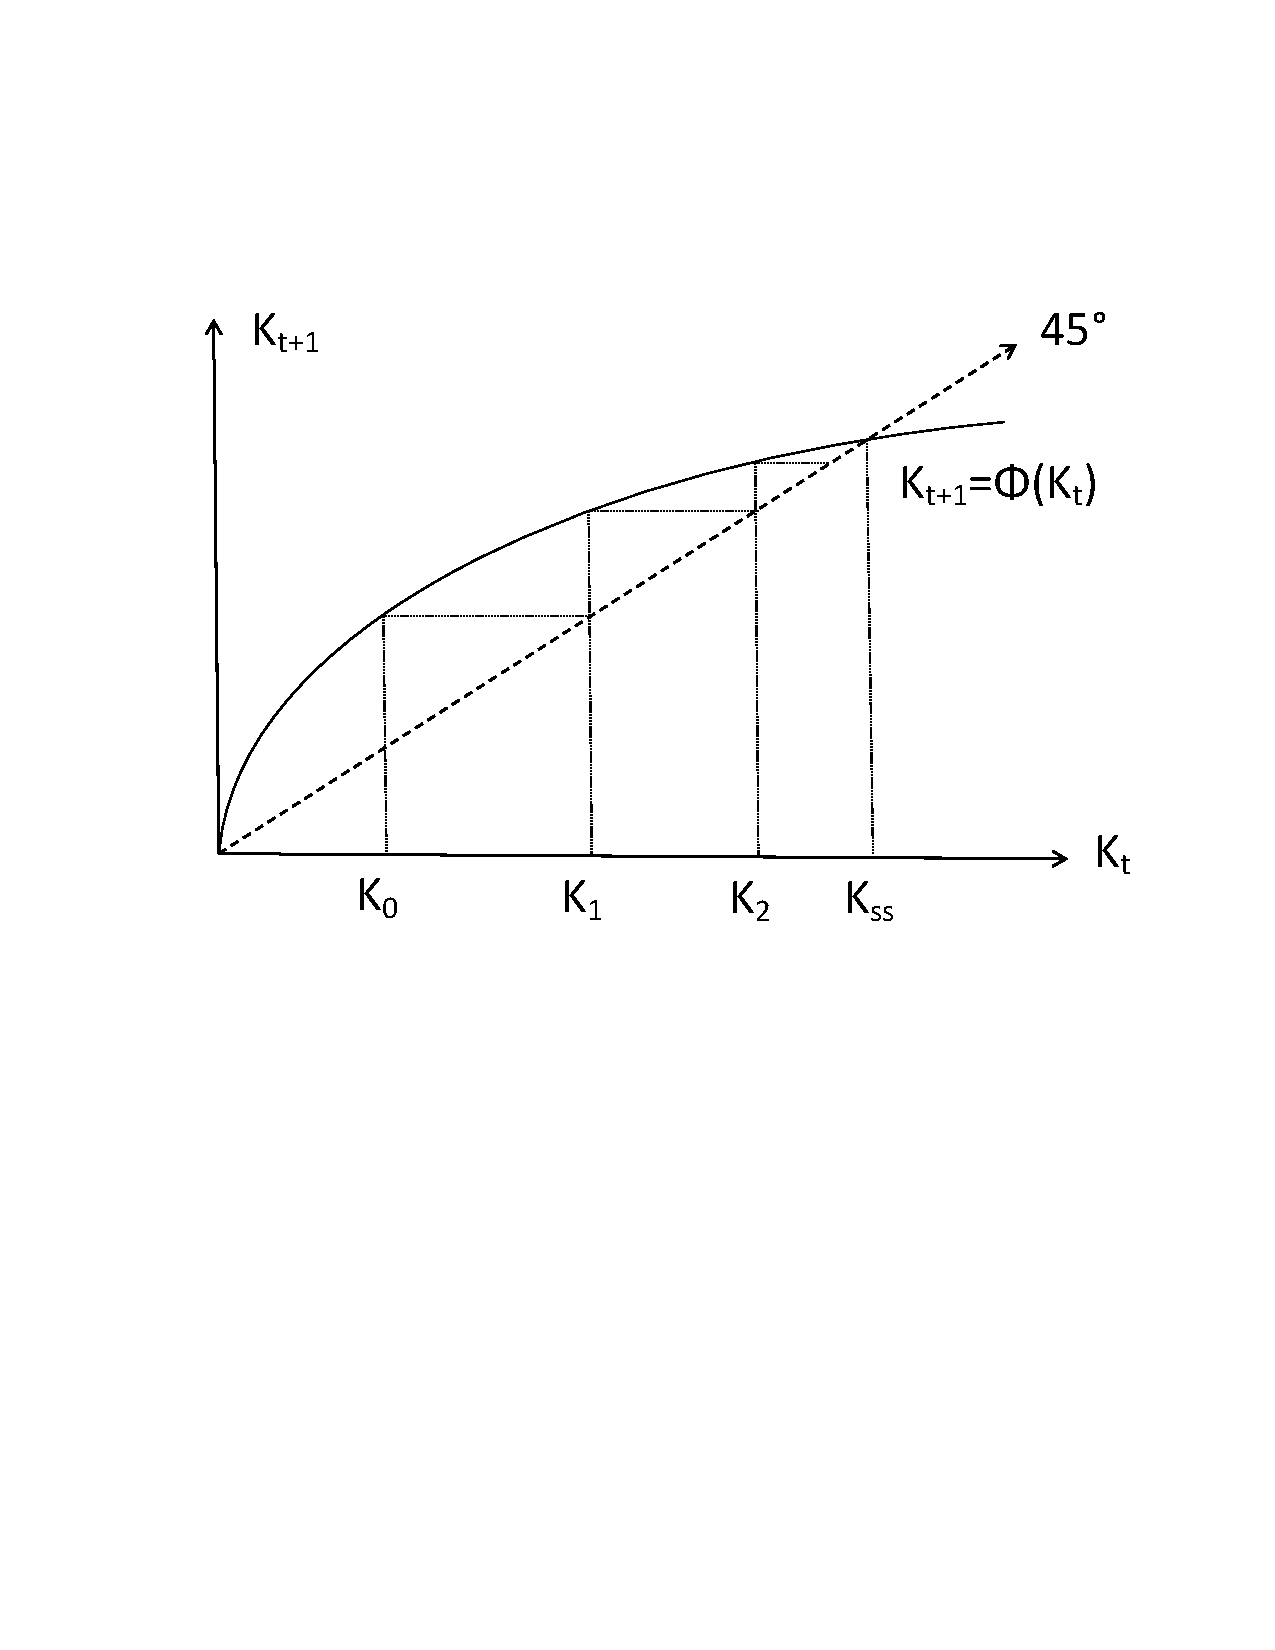
\includegraphics{DSGE_Solow1_Fig.pdf}}}
			\end{figure}

			Suppose we started off the economy with a capital stock of $K_0$. The policy function, $K_{t+1}=\Phi(K_t)$ gives a value of $K_1$ for next period. Then, next period, the policy function gives $K_2$, and so forth. In the long run the capital stock will converge to $K_{ss}$, the steady state value.

			Since there are no stochastic shocks in this model, the state is described by a single variable, $K_t$. The dynamics of this model are such that the capital stock converges over time to its steady state value and then stays there forever.

			If we allow for stochastic shocks, there is no steady state, at least not in the same sense. Suppose we have a different production function for the Solow model that allowed for a stochastic shock to productivity.
			\begin{equation}
			Y_t = K_t^\alpha (L_te^{z_t})^{1-\alpha} \nonumber
			\end{equation}

			Further suppose that the shock takes on one of two values randomly.
			\begin{equation}
			z_t = \left\{\begin{matrix} z_1 & \text{with probability  } \pi \\ z_2 & \text{with probability  } 1-\pi \end{matrix} \right. \nonumber
			\end{equation}

			The policy function becomes
			\begin{equation}
			 K_{t+1} = (1-\delta)K_t  + s K_t^\alpha e^{(1-\alpha)z_t}
			\end{equation}

			Figure \ref{DSGE_Solow2_Fig} plots this.
			\begin{figure}[htb]\centering \captionsetup{width=4.0in}
			   \caption{\label{DSGE_Solow2_Fig}\textbf{Policy Function and Steady State for the Solow Model}}
			   \fbox{\resizebox{5.0in}{3.5in}{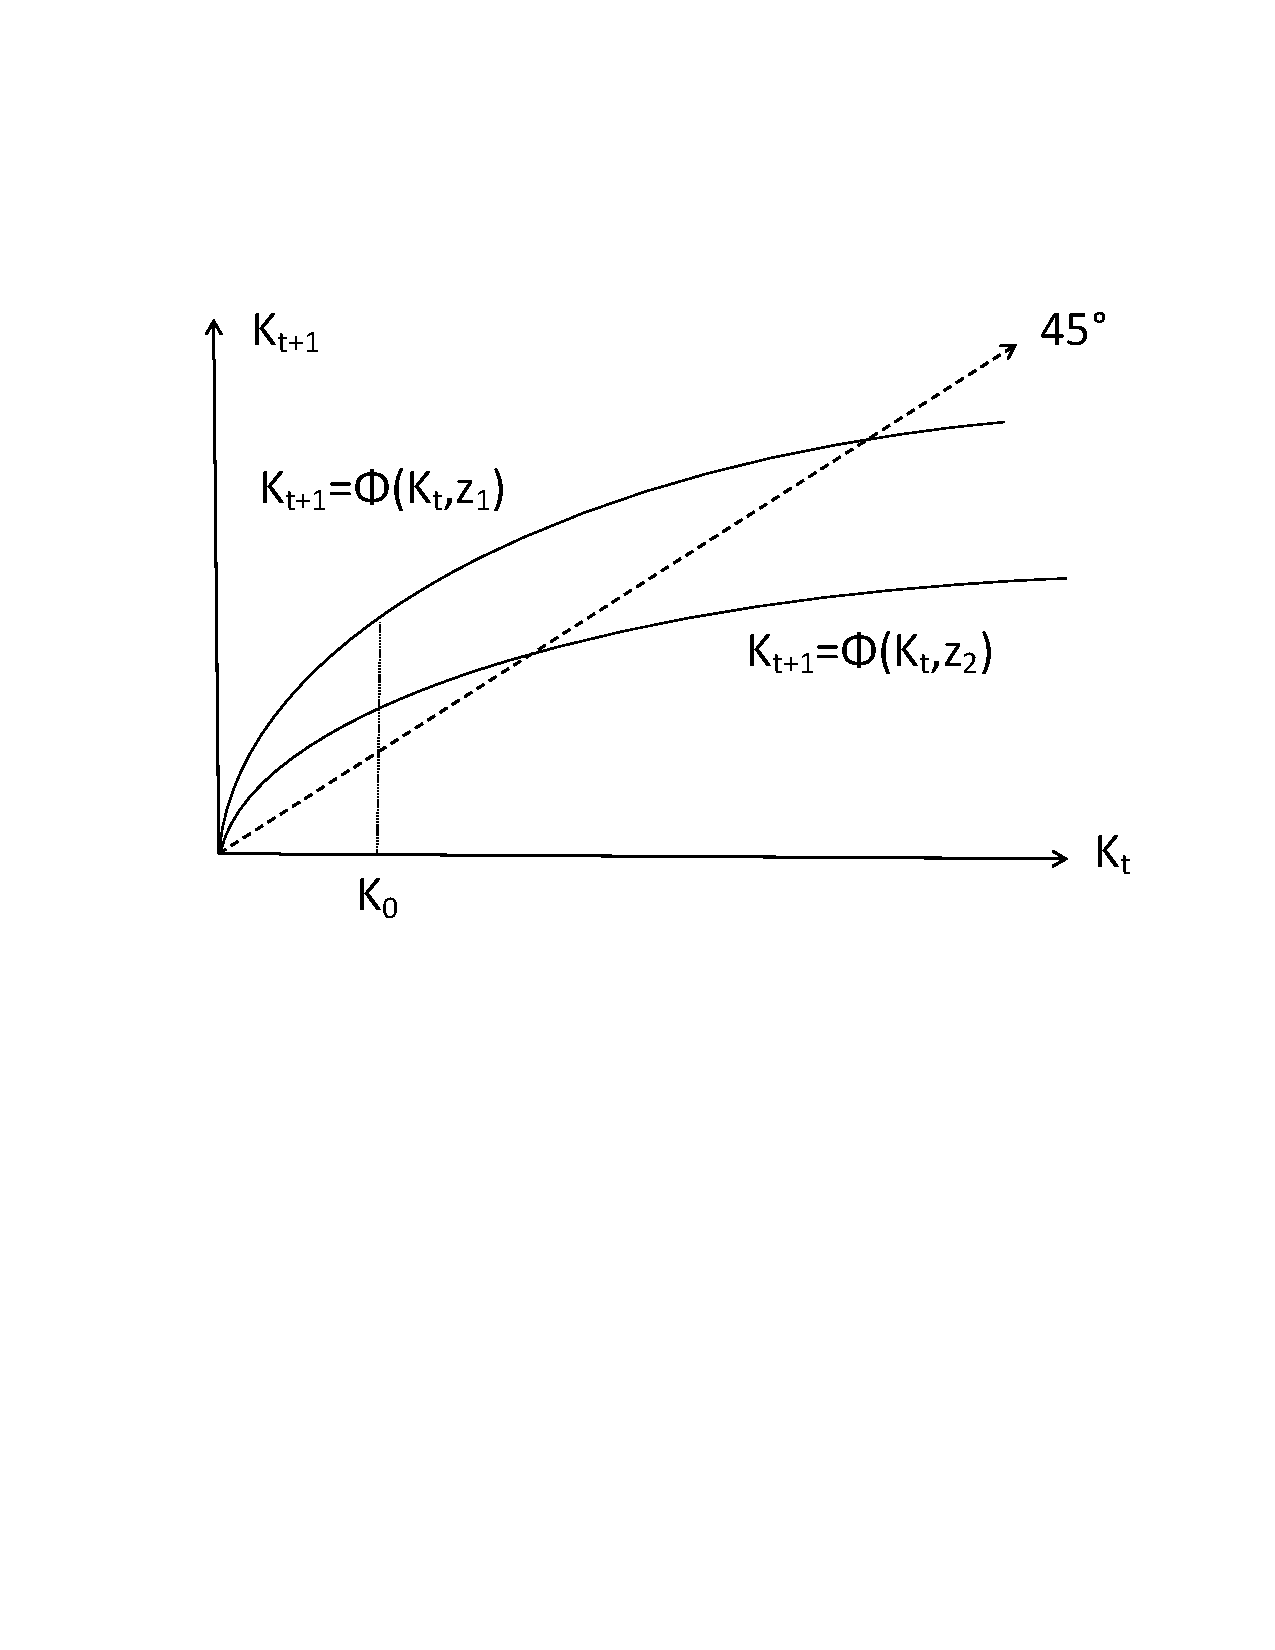
\includegraphics{DSGE_Solow2_Fig.pdf}}}
			\end{figure}
			Because there are two policy functions and the economy switches randomly between these two, there is no steady state in the sense of a constant long-run value. However, in the long run, the state of economy does settle down to a constant \emph{distribution} for the capital stock. This distribution is referred to as the ``ergodic" distribution and the economy is said to be in a ``stationary" state.

			Often we talk about the ``steady state" of a stochastic model. When we do, we are referring to a counter-factual state that economy will not ever reach or maintain. This steady state is defined as the value for the state variables toward which the economy would trend, if the stochastic shock were permanently at its steady state value. Another way to think of this is that it is the steady state for a non-stochastic version of the model, where the innovations to the stochastic shocks (the $\epsilon^z$'s) are always zero.

			To solve for the steady state we set all stochastic shocks to their long run value and do the same for the endogenous state variables.

			In the stochastic Solow model we get:
			\begin{equation}
			 \bar K = (1-\delta)\bar K  + s \bar K^\alpha e^{(1-\alpha)\bar z}  ; \quad \bar z = \pi z_1 + (1-\pi)z_2
			\end{equation}

			The solution for $\bar K$ is:
			\begin{equation}
			\bar K = \left(\frac{se^{(1-\alpha)\bar z}}{\delta}\right)^{\frac{1}{1-\alpha}}
			\end{equation}

			%\FloatBarrier

		%section 4
		\subsubsection{Brock and Mirman's Model} \label{DSGE_BrockMirman}
			In this section we build a variant of the model in \citet{BrockMirman1972}.  This model is absurdly simple, but is valuable for two reasons.  First, the closed-form solution for the policy function is known.   And second, it is an easy model to use when illustrating our numerical techniques later in the course.

			Households solve the followng dynamic program.
			\begin{equation}\label{DSGE_BMBellman}
			V(K_t,z_t) = \max_{K_{t+1}}\ln (e^{z_t}K_t^\alpha - K_{t+1}) + \beta E_t\{V(K_{t+1},z_{t+1})\}
			\end{equation}
			The associated Euler equation is:
			\begin{equation}\label{DSGE_BMEuler}
			\frac{1}{e^{z_t}K_t^\alpha - K_{t+1}} = \beta E_t \left\{\frac{\alpha e^{z_{t+1}}{K_{t+1}}^{\alpha-1}}{e^{z_{t+1}}{K_{t+1}}^\alpha - K_{t+2}} \right\}
			\end{equation}
			The law of motion for $z$ is:
			\begin{equation}\label{LOM}
			z_{t+1} = \rho z_t + \ve_t; \quad \ve_t \sim i.i.d(0,\sigma^2)
			\end{equation}
			
			You be we asked in an exercise at the end of this chapter to verify that the policy function takes the following form:
			\begin{equation}\label{DSGE_BMpolicy}
			K_{t+1} = A e^{z_t}K_t^\alpha
			\end{equation}
			You will need to find the value of $A$ as a function of the model's parameters.

			The steady state value of $K$ is defined by using \eqref{DSGE_BMpolicy} with $K_t=K_{t+1}$ and $z_t=0$.
			\begin{equation}\label{DSGE_BMSSK}
			\bar K = A ^\frac{1}{1-\alpha}
			\end{equation}

			The parameters of the model are, $\alpha$, $\beta$, $\rho$ and $\sigma$.  When values are needed for numerical calculations use the following default values unless otherwise indicated:
			\begin{equation}\label{parameters}
			\begin{split}
			\alpha & = .35 \\
			\beta & = .98 \\
			\rho & = .95 \\
			\sigma & = .02 \\ \nonumber
			\end{split}
			\end{equation}

		%subsubsection 3.7.2
		\subsubsection{Steady State of the Baseline Model}\label{DSGE_SS_Base}
			To find the steady state in our DSGE model we need to proceed similarly and replace the time-period-specific values of$\{c_t,k_t,\ell_t,w_t,r_t,\tau_t\>\&\>z_t\}$ in \eqref{DSGE_BC22HouseholdSpec} -- \eqref{DSGE_LoM2Spec} with their steady state values as below:
			\begin{equation}\label{DSGE_BC23HouseholdSpec}
			\bar c = (1-\tau) \left[\bar w \bar \ell+(\bar r-\delta)\bar k\right] + \bar T
			\end{equation}
			\begin{equation}\label{DSGE_Euler23HouseholdDSGE}
			u_c(\bar c,\bar \ell) = \beta E_t\left\{ u_c(\bar c,\bar \ell)[(\bar r-\delta)(1-\tau)+1] \right\}
			\end{equation}
			\begin{equation}\label{DSGE_EulerB3HouseholdSpec}
			-u_{\ell}(\bar c,\bar \ell) = u_{c}(\bar c,\bar \ell)\bar w(1-\tau)
			\end{equation}
			\begin{equation}\label{DSGE_FOC013FirmSpec}
			\bar r = f_K(\bar k,\bar \ell,\bar z)
			\end{equation}
			\begin{equation}\label{DSGE_FOC023FirmSpec}
			\bar w = f_L(\bar k,\bar \ell,\bar z)
			\end{equation}
			\begin{equation}\label{DSGE_GovtBC3FirmSpec}
			\tau \left[\bar w \bar \ell+(\bar r-\delta)\bar k\right] = \bar T
			\end{equation}

			\eqref{DSGE_BC23HouseholdSpec} -- \eqref{DSGE_GovtBC3FirmSpec} implicitly define a steady state via a system of six equations in six unknowns, the unknowns being $\bar k, \bar c, \bar w, \bar r, \bar \ell$ and $\bar T$ \eqref{DSGE_BC23HouseholdSpec} and \eqref{DSGE_GovtBC3FirmSpec} can be used as definitions, reducing the system to four equations in $\bar k, \bar w, \bar r$ and $ \bar \ell$ .

			With this system we could perform comparative statics on the steady state by totally differentiating the remaining four equations: \eqref{DSGE_Euler23HouseholdDSGE}, \eqref{DSGE_EulerB3HouseholdSpec}, \eqref{DSGE_FOC013FirmSpec} and \eqref{DSGE_FOC023FirmSpec}, using the chain rule on equations \eqref{DSGE_BC23HouseholdSpec} and \eqref{DSGE_GovtBC3FirmSpec} as needed. Exercise 7 requires such a task.

			To proceed further we need functional forms for $u(c,\ell)$ and $f(k,\ell,z)$. If we choose appropriate functional forms it will be possible to solve explicitly for the steady state value of $k$ as a function of the parameters. Taking comparative statics is relatively easy for $\bar k$. Once this is known we can substitute it back into equations \eqref{DSGE_BC23HouseholdSpec} -- \eqref{DSGE_GovtBC3FirmSpec} appropriately to get the comparative statics for all the other steady state variables.

	%subsection 3.8
	\subsection{Additional Issues}\label{DSGE_AdditionSpec}
		Finally note that we have nowhere in our DSGE model defined other common variables such as investment and GDP. We can easily do so, however, by adding additional definitional equations. For example, GDP would be given by:
		\begin{equation}
		y_t = f(k_t,\ell_t,z_t)
		\end{equation}

		Investment is given by:
		\begin{equation}
		i_t =k_{t+1} - (1-\delta)k_t
		\end{equation}

		In addition, while $r_t$ is the rental rate on capital, it is not the same as the real interest rate that would be offered on financial assets. The closest analog is the \it user cost of capital\rm, which is defined as:
		\begin{equation}
		u_t = r_t - \delta
		\end{equation}

		Other variables of interest can be defined in similar ways. Once steady state values are found for the state variables (in our case $\bar k$ and $\bar z$) we can find the steady state values of all other variables in the model.

		Also note that the state can be expanded to include variables that are not necessary to define the state. For example, if we cannot rewrite one of the equations so that $\ell_t$ is isolated as a definition, we would still have an equation or set of equations that implicitly define its value. In this case if often turns out to be useful to simply include $\ell_t$ in the set of endogenous state variables even though it is not strictly a state variable. Indeed we will see that in some cases it is best to treat all the variables in the model as if they were state variables (this is the case with the DSGE modeling program, Dynare, for example). This means that it is perfectly legitimate to rewrite \eqref{DSGE_XYZSpec} as \eqref{DSGE_XYZ2Spec} or \eqref{DSGE_XYZ3Spec}.

		\begin{equation}\label{DSGE_XYZ2Spec}
		\begin{aligned}
		& X_t  = \left\{k_{t-1},\ell_t\right\} \\
		& Y_t  = \left\{c_t,w_t,r_t,T_t\right\} \\
		& Z_t  = \left\{z_t\right\} \\
		\end{aligned}
		\end{equation}

		\begin{equation}\label{DSGE_XYZ3Spec}
		\begin{aligned}
		& X_t = \left\{k_{t-1},\ell_t,c_t,w_t,r_t,T_t\right\} \\
		& Y_t = \emptyset \\
		& Z_t = \left\{z_t\right\} \\
		\end{aligned}
		\end{equation}

%section 5
\section{Introduction to Solution Methods}\label{DSGE_Solutions}
	Except for a few known special cases, it is generally impossible to solve algebraically for the policy function in a DSGE model.  One case where it is possible is given in Exercise 1.  This means we must resort to numerical techniques to solve and simulate DSGE models. The set of solution techniques that have been used in the past includes:

	\begin{itemize}
	\item discrete grid approximations
	\item spline function approximations
	\item linear-quadratic approximations objective functions and constraints
	\item log-linearization of the characterizing equations
	\item higher-order approximation of the characterizing equations
	\end{itemize}

	We will discuss all of these, but will go into special detail with the last two methods

	%subsection 5.1
	\subsection{Grids and Splines}\label{DSGE_GridSplineSoll}
		Discrete grid methods are very computationally intensive, but can be ideal for highly nonlinear policy functions.  In our DSGE model the policy function is $k_{t+1} = \Phi(k_t,z_t)$.  To approximate this with a discrete grid, we would set up a support for $k$ and $z$ with a finite number of elements (the grid).  To find the policy function, for every combination of the values for $k_t$ and $z_t$ in the grid, we would find the value of $k_{t+1}$ in the finite support of $k$ that comes closet to satisfying the general equilibrium conditions.  If there are $N$ elements in the support of $k$ and $M$ elements in the support of $z$, then the policy function is an $N\times M$ array with an index number in each element of the array indicating which of the $N$ elements in the support of $k$ is optimal.  Figure \ref{DSGE_Grid_Fig} illustrates this discretized policy function for a particular value of $z$, $z_0$.

		\begin{figure}[htb]\centering \captionsetup{width=4.0in}
		   \caption{\textbf{Grid Approximation to the True Policy Function}}
		   \label{DSGE_Grid_Fig}
		   \fbox{\resizebox{5.0in}{3.5in}{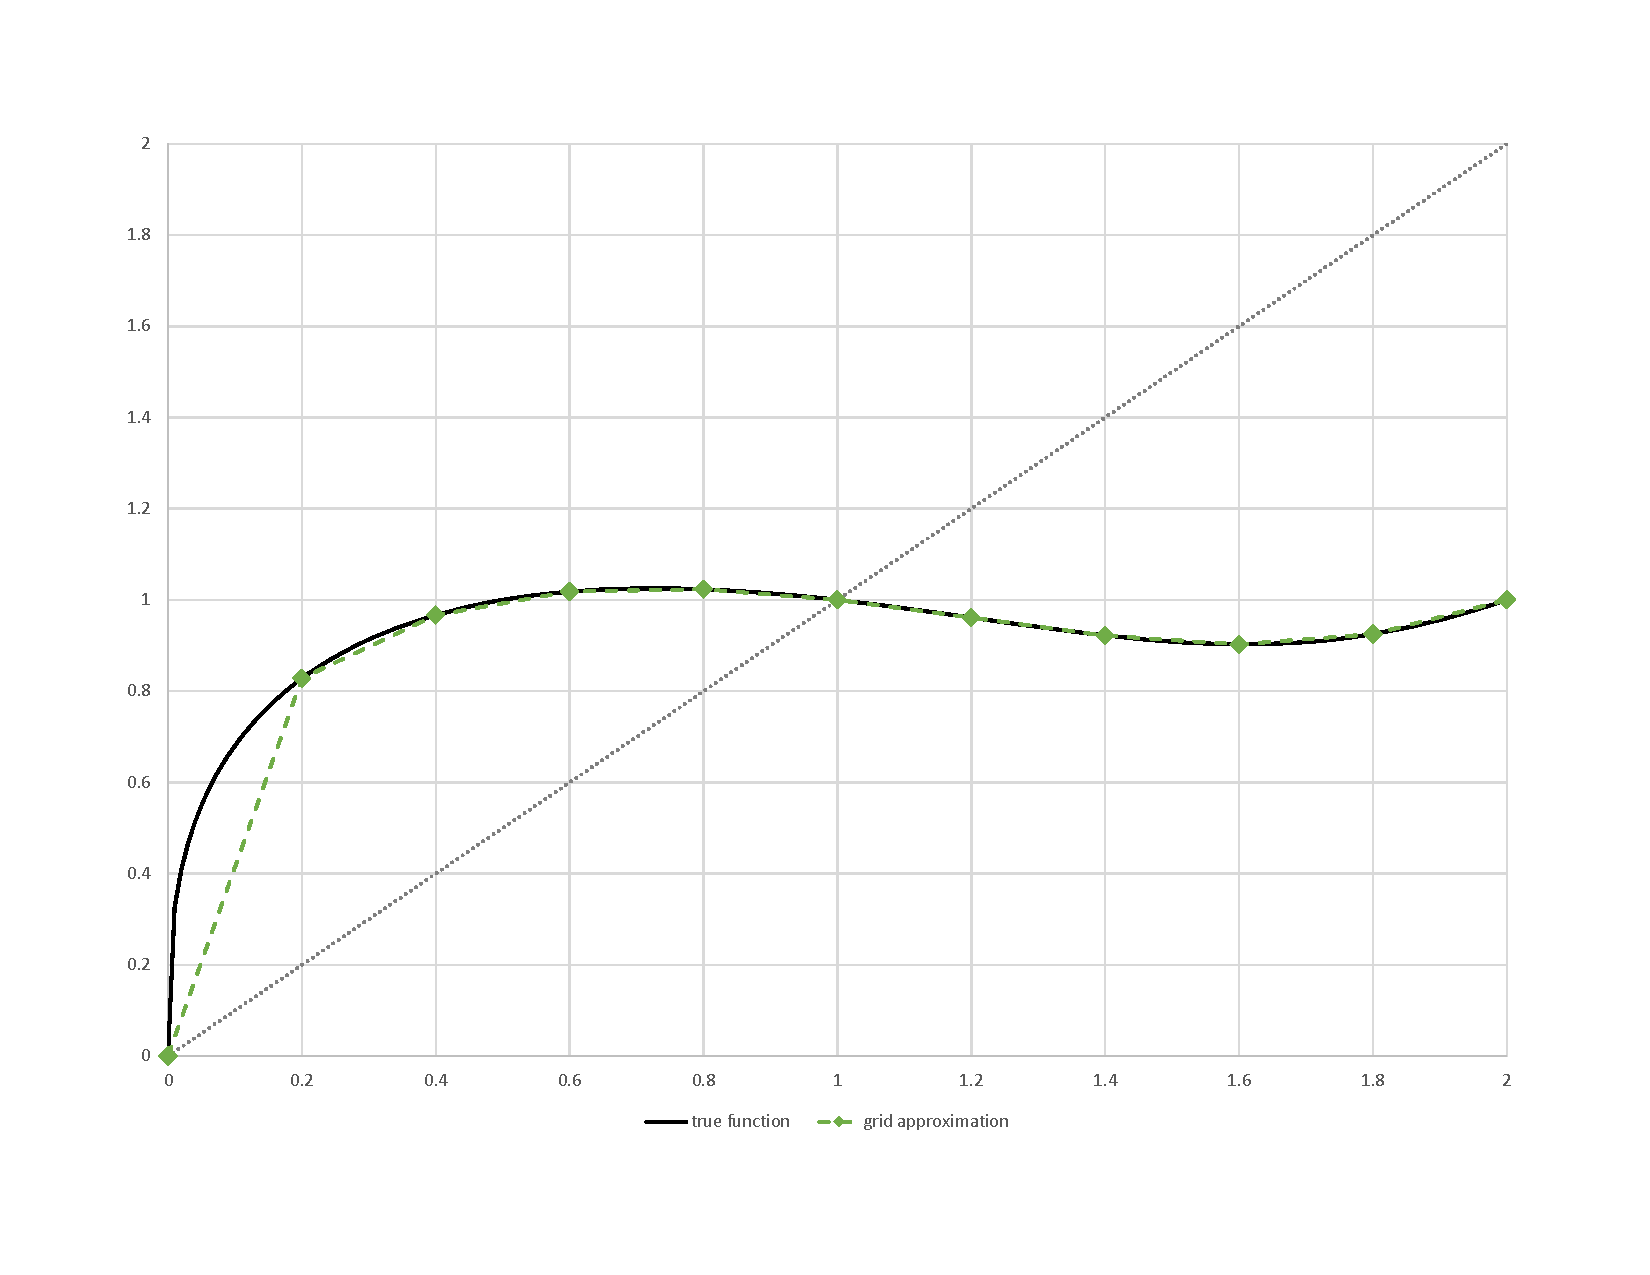
\includegraphics{DSGE_Grid_Fig.pdf}}}
		\end{figure}

		As the grid becomes finer with more elements in the supports, the approximation becomes better.

		A spline approximation allows us to fill in the values between the discrete points on the support.  Simple splines could be linear, or they could be curved to approximate smooth functions better using a quadratic or cubic function over the interval between the points.

		There is a great deal of literature on the optimal grid structure and the optimal splines for approximation in a variety of settings.  Engineering applications often use these tools.  In economics they are less widely used, most likely because the behavior of many DSGE models is quite smooth making other approximation techniques computationally more efficient.

	%subsection 5.2
	\subsection{Blanchard-Kahn and Linear-Quadratic Methods}\label{LinQuadSol}
		One of the first approximation methods to be used with DSGE models was introduced by \citet{BlanchardKahn1980} who adapted numerical techniques from the engineering literature.  An excellent discussion of this is given in \citet[pp. 129-132]{McCandless2008}.

		Another early method employed by \citet{KydlandPrescott1982} is to optimize an objective function that is approximated by a quadratic, subject to linear constraints.  This is usually the household's utility function maximized subject to a budget constraint.  Intuitively, since the objective is quadratic, the Euler equations derived will be linear yielding highly tractable equations from which to derive a solution.  In terms of our baseline DSGE model we take a quadratic approximation of the utility function in \eqref{DSGE_VFHouseholdSpec} and then use the first-order conditions to derive specific versions of equations \eqref{DSGE_Euler2HouseholdSpec} and \eqref{DSGE_EulerBHouseholdSpec}.  These will be simple linear equations and the system can be solved following the steps outlined in \citet[ch. 7]{McCandless2008}.

	%subsection 5.3
	\subsection{Log-Linearization Methods}\label{LogLinSol}
		The best sources here are \citet{Uhlig1999} and \citet{Christiano2002}.  Log-linearization will be covered in excruciating detail in the next chapter.  Here we will simply note the intuition.  Rather than approximate the objective function as above, log-linearization techniques involve taking approximations of the final characterizing equations.  In terms of our DSGE model from \ref{DSGE_BaselineDSGE} we would take logs of equations \eqref{DSGE_BC22HouseholdSpec} -- \eqref{DSGE_GovtBC2FirmSpec} and then take linear approximations of these, almost always by taking a first-order Taylor-series expansion of the equations.  If we assume the policy function is also log-linear then some straightforward algebra yields its coefficients.  Numerically solving for these coefficients can be challenging, particularly if the state space of the model is large.

		The Taylor-series expansion requires a point about which the functions are approximated.  In almost all cases this is the steady state of the model.  Most models are stable and well-behaved and the stationary state is one where the state fluctuates around in a neighborhood near the zero-innovation steady state.  \citet{EvansPhillips2014} show how linearizing about a different point may improve the approximation for models that are unstable or which are for other reasons rarely in the neighborhood of the steady state.

	%subsection 5.4
	\subsection{Perturbation Methods}\label{PertSol}
		Log-linearization methods will be very good approximations in the neighborhood of the expansion point.  One way to improve the accuracy of the approximation is to incorporate higher-order terms from the Taylor-series expansion of the characterizing equations.  Higher-order terms means finding greater numbers of coefficients.  The classic citation for the numerical method of finding higher-order coefficients is \citet{Judd1992} and the method is referred to a the ``perturbation method."

		Consider our intertemporal Euler equation from \eqref{DSGE_Euler2HouseholdSpec}, reproduced below.
		\begin{equation}
		u_c(c_t,\ell_t) = \beta E_t\left\{ u_c(c_{t+1},\ell_{t+1})[(r_{t+1}-\delta)(1-\tau)+1] \right\}
		\end{equation}
		Note that the right-hand side of the equation involves taking an expectation.  If we linearize or log-linearize this equation, the expectations operator passes through and we end up with linear equations in the expected values of the variables.  This generates a phenomenon known as ``certainty equivalence" which will not hold generally.  The right-hand side takes the expectation of the marginal utility of consumption times a rate of return on capital.  By log-linearizing this becomes equal to the marginal utility of the expected consumption times the expected return on capital.  These are only approximately the same.  And the difference can be important if we are dealing with things like risk aversion and risk premia.  For this reason, higher-order approximations are a must when dealing with models where riskiness is a central feature of the model.

		\begin{figure}[htb]\centering \captionsetup{width=4.0in}
			\label{DSGE_Poly_Fig}
		   \caption{\textbf{Polynomial Approximations to the True Policy Function}}
		   \fbox{\resizebox{5.0in}{3.5in}{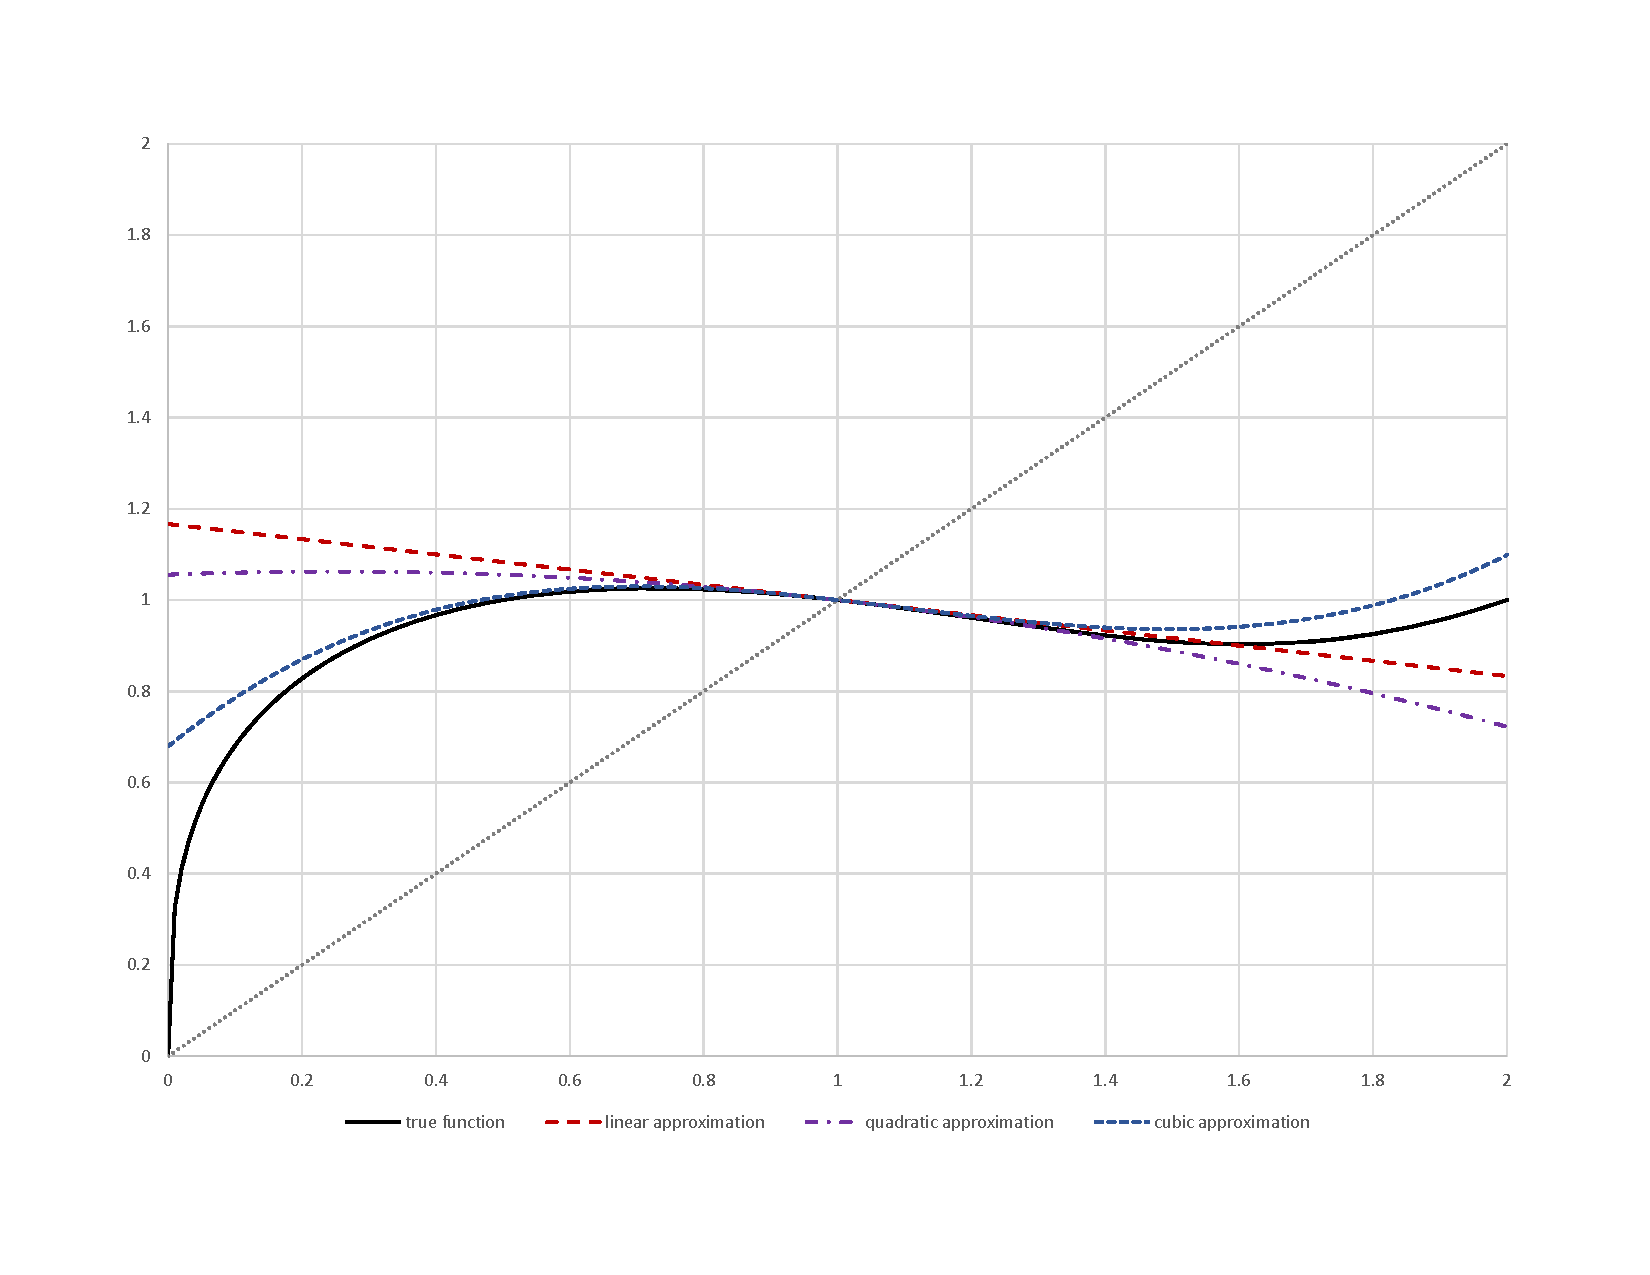
\includegraphics{DSGE_Poly_Fig.pdf}}}
		\end{figure}

	%subsection 5.5
	\subsection{GSSA}\label{GSSA}
		More recently \citet{Juddetal2011} have introduced a computational technique which they call a ``generalized stochastic simulation algorithm'' (GSSA) that gives very good approximations to policy functions.  This techniques does not require the imposition of certainty equivalence and are suitable for a large variety of dynamic general equilibrium models.  The technique involves estimating a non-linear function with sufficient flexibility in the parameters that it describes the true function well for the range of values actually encountered in the simulation.  We will discuss this method later in the course.

	%subsection 5.6
	\subsection{Linearizing about the Current State}\label{CSL}
		\citet{EvansPhillips2014} have a technique that closely approximates policy functions by linearizing each period about the current state of the economy, rather than the steady state.  Their solutions are not exact and introduce what they refer to as ``isolation'' error, but it eliminates entirely the mismatch between a polynomial approximation and the true function due to distance from the approximation point.  They show that their technique is very accurate and computationally less burdensome than grid methods.

		\begin{figure}[htb]\centering \captionsetup{width=4.0in}
			\label{DSGE_CSL_Fig}
		   \caption{\textbf{Approximation by Linearization about the Current State}}
		   \fbox{\resizebox{5.0in}{3.5in}{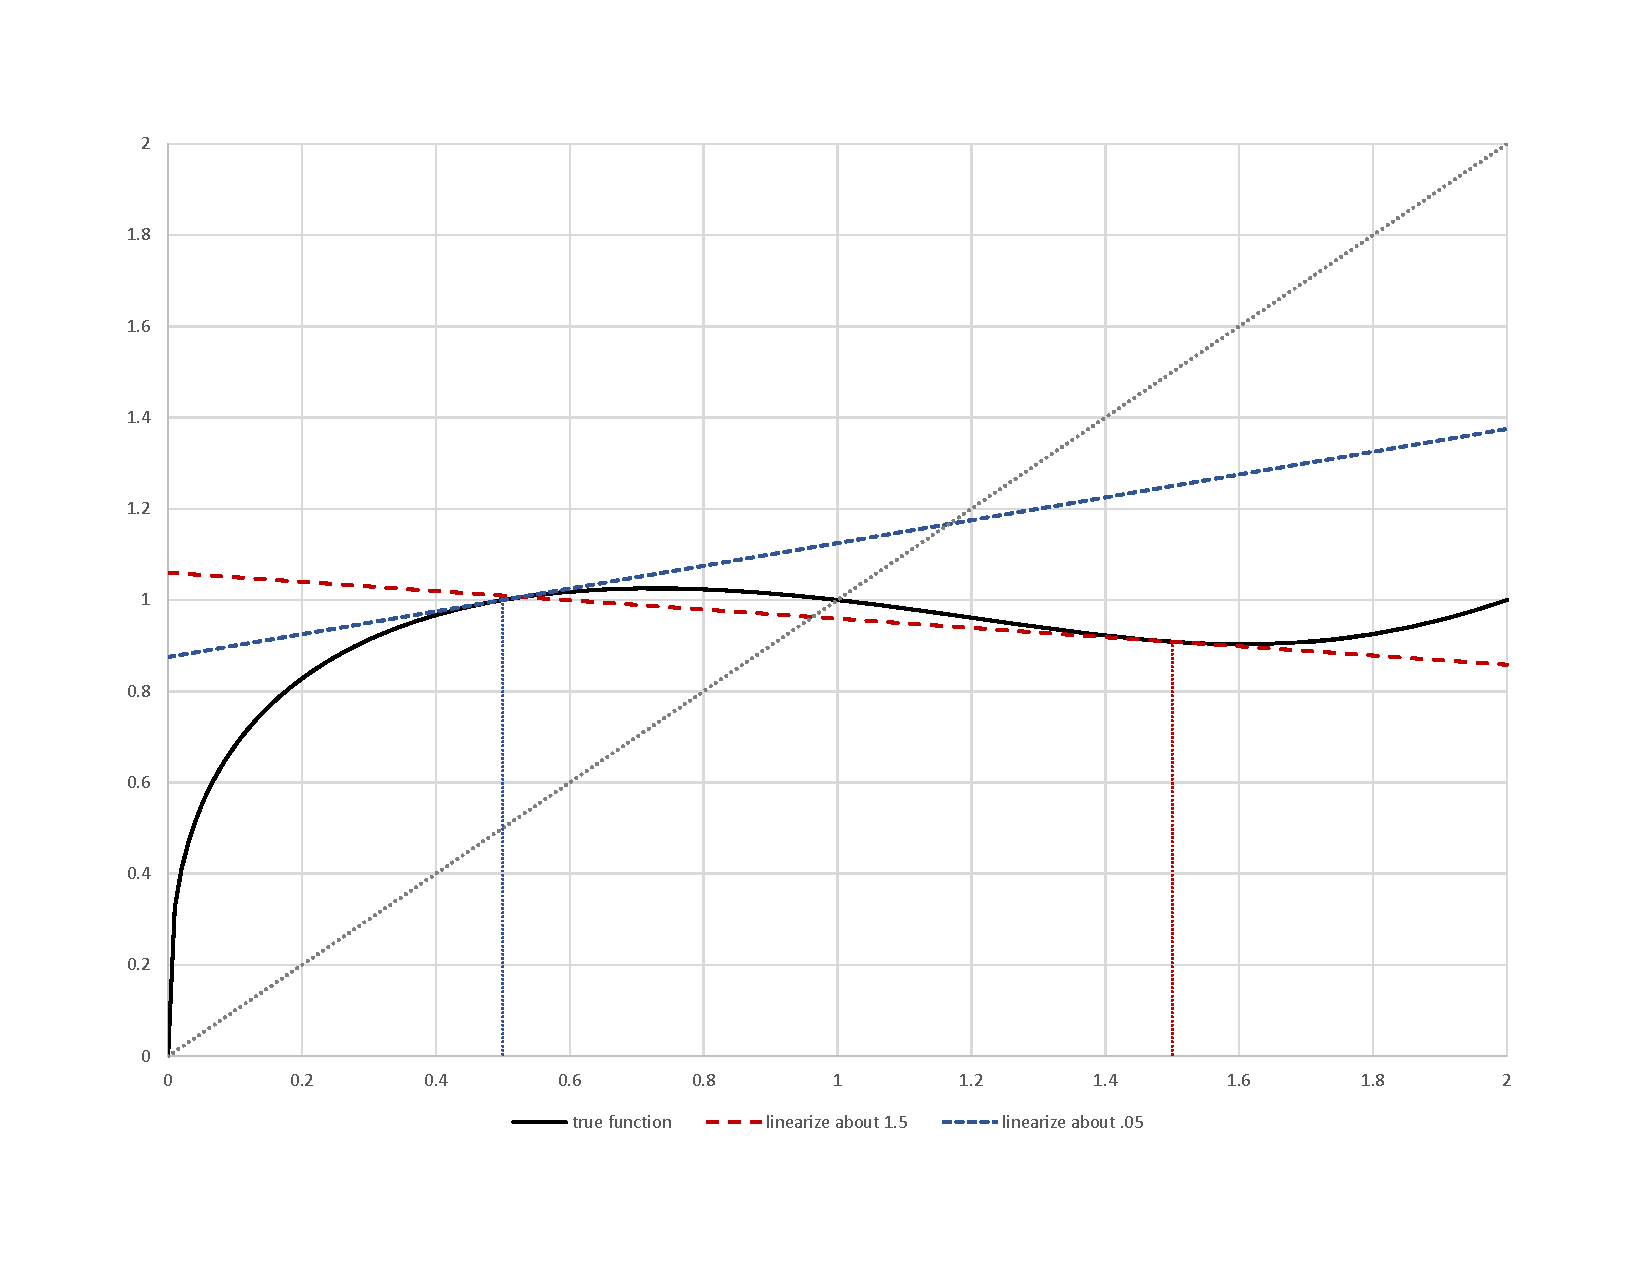
\includegraphics{DSGE_CSL_Fig.pdf}}}
		\end{figure}

%Exercises
\newpage
\section*{Exercises}\label{DSGE_HW}

	% 1
	\begin{exercise} \label{DSGE_HW_BM_FindA}
		For the Brock and Mirman model, find the value of $A$ in the policy function.  Show that your value is correct.

		For this case find an algebraic solution for the policy function, $k_{t+1} = \Phi (k_t,z_t)$.  Couple of good sources for hints are \citet[exercise 2.2, p. 12]{StokeyLucas1989} and \citet[exercise 1.1, p. 47]{Sargent1987}.
	\end{exercise}

	% 2
	\begin{exercise} \label{DSGE_HW_CharEq_Ln}
		For the model in section \ref{DSGE_BaselineDSGE} of the notes consider the following functional forms:
		\begin{equation}\label{DSGE_HW_CharEq_Ln_eq01}
		\begin{split}
		u(c_t,\ell_t) & = \text{ln }c_t + a \text{ ln }(1-\ell_t)\\
		F(K_t,L_t,z_t) & = e^{z_t}K^{\alpha}_t L^{1-\alpha}_t  \nonumber
		\end{split}
		\end{equation}
		Write out all the characterizing equations for the model using these functional forms.

		Can you use the same tricks as in Exercise 1 to solve for the policy function in this case?  Why or why not?
	\end{exercise}

	% 3
	\begin{exercise} \label{DSGE_HW_CharEq_CES_Ln}
		For the model in section \ref{DSGE_BaselineDSGE} consider the following functional forms:
		\begin{equation}\label{DSGE_HW_CharEq_CES_Ln_eq01}
		\begin{split}
		u(c_t,\ell_t) & = \frac{c^{1-\gamma}_t -1}{1-\gamma}+ a \text{ ln }(1-\ell_t)\\
		F(K_t,L_t,z_t) & = e^{z_t}K^{\alpha}_t L^{1-\alpha}_t  \nonumber
		\end{split}
		\end{equation}
		Write out all the characterizing equations for the model using these functional forms.
	\end{exercise}

	% 4
	\begin{exercise} \label{DSGE_HW_CharEq_CES}
		For the model in section \ref{DSGE_BaselineDSGE} consider the following functional forms:
		\begin{equation}\label{DSGE_HW_CharEq_CES_eq01}
		\begin{split}
		u(c_t,\ell_t) & = \frac{c^{1-\gamma}_t -1}{1-\gamma}+ a \frac{(1-\ell_t)^{1-\xi}-1}{1-\xi}      \\
		F(K_t,L_t,z_t) & = e^{z_t}\left[\alpha K^{\eta}_t +(1-\alpha)L^{\eta}_t \right]^{\frac{1}{\eta}}   \nonumber
		\end{split}
		\end{equation}
		Write out all the characterizing equations for the model using these functional forms.
	\end{exercise}

	% 5
	\begin{exercise} \label{DSGE_HW_NoLeisure}
		For the model in section \ref{DSGE_BaselineDSGE} abstract from the labor/leisure decision and consider the following functional forms:
		\begin{equation}\label{DSGE_HW_NoLeisure_eq01}
		\begin{split}
		u(c_t) & = \frac{c^{1-\gamma}_t -1}{1-\gamma}      \\
		F(K_t,L_t,z_t) & = K^{\alpha}_t (L_te^{z_t})^{1-\alpha}  \nonumber
		\end{split}
		\end{equation}
		Write out all the characterizing equations for the model using these functional forms.  Assume $\ell_t=1$.

		Write out the steady state versions of these equations.  Solve algebraically for the steady state value of $k$ as a function of the steady state value of $z$ and the parameters of the model.  Numerically solve for the steady state values of all variables using the following parameter values: $\gamma = 2.5$, $\beta = .98$, $\alpha = .40$, $\delta = .10$, $\bar z = 0$ and $\tau = .05$.  Also solve for the steady state values of output and investment.  Compare these values with the ones implied by the algebraic solution.
	\end{exercise}

	% 6
	\begin{exercise} \label{DSGE_HW_CES}
		For the model in section \ref{DSGE_BaselineDSGE} consider the following functional forms:
		\begin{equation}\label{DSGE_HW_CES_eq01}
		\begin{split}
		u(c_t,\ell_t) & = \frac{c^{1-\gamma}_t -1}{1-\gamma}+ a \frac{(1-\ell_t)^{1-\xi}-1}{1-\xi}      \\
		F(K_t,L_t,z_t) & = K^{\alpha}_t (L_te^{z_t})^{1-\alpha}  \nonumber
		\end{split}
		\end{equation}
		Write out all the characterizing equations for the model using these functional forms.  {}Write out the steady state versions of these equations.  Numerically solve for the steady state values of all variables using the following parameter values: $\gamma = 2.5$, $\xi = 1.5$,  $\beta = .98$, $\alpha = .40$, $a=.5$, $\delta = .10$, $\bar z = 0$, and $\tau = .05$.  Also solve for the steady state values of output and investment.
	\end{exercise}

	% 7
	\begin{exercise} \label{DSGE_HW_Base_TotalDiff}
		For the steady state of the baseline tax model in section \ref{DSGE_SS_Base} use numerican differentiation to solve for the full set of comparative statics and sign them where possible.  Find $\frac{\partial y}{\partial x}$ for $y\in\{\bar k, \bar \ell, \bar y, \bar w, \bar r, \bar T, \bar i, \bar c \}$ and $x\in\{\alpha, \beta, \gamma, \delta, \xi, \tau, a, \bar z\}$.

		Using the same parameter values as in excercise \ref{DSGE_HW_CES}, solve for the numerical values of the comparative statics.
	\end{exercise}

	%8
	\begin{exercise} \label{DSGE_HW_BM_Grid}
		For the Brock and Mirman model in section \eqref{DSGE_BrockMirman} set up a discrete grid for $K$ with 25 values ranging from $.5 \bar K$ to $1.5 \bar K$.  Also set up a discrete grid for $z$ with 25 values ranging from $-5\sigma$ to $+5\sigma$.  Set up a value function array, $V$ that stores the value for all $26^2$ possible permutations of $K$ and $z$.  Also set up a policy function array, $H$, that stores the optimal index value of $K'$ for all all $25^2$ possible permutations of $K$ and $z$.

		To begin assume that all elements of $V$ are zero and that all elements of $H$ point to the lowest possible value for $K$ ($.5 \bar K$).

		Loop over all possible values of $K$ and $z$ and for each combination find 1) the optimal value of $K'$ from the 25 possible values.  Store this value in an updated policy function array, $H_{new}$.  Also find 2) the value implied by this choice given the current value function.  Store this in an updated value function array, $V_{new}$.

		Once this is completed for all $K$ and $z$ check to see if $V$ is approximately equal to $V_{new}$.  If so, output the value function and policy function arrays.  If not, replace $V$ with $V_{new}$ and $H$ with $H_{new}$ and repeat the search above.

		When finished plot the three-dimensional surface plot for the policy function $K' = H(K,z)$.  Compare this with the closed form solution as described in section \ref{DSGE_BrockMirman}.
	\end{exercise}

	%9
	\begin{exercise} \label{DSGE_HW_BM_Grid_Log}
		Repeat the above exercise using $k \equiv \ln K$ in place of $K$ as the endogenous state variable.
	\end{exercise}

	% %10
	% \begin{exercise} \label{DSGE_HW_Base_Grid_Log}
	% 	Repeat the exercise \ref{DSGE_HW_BM_Grid} for the baseline tax model in section \ref{DSGE_SS_Base} using the same parameter values as in Exercise \ref{DSGE_HW_CES}.
	% \end{exercise}

	% %11
	% \begin{exercise} \label{Linear_HW_Base_Sims}
	% 	For the same model as above, generate 10,000 artificial time series for an economy where each time series is 250 periods long.  Start each simulation off with a starting value for $k$ equal to the steady state value, and a value of $z=0$.

	% 	Use $\sigma_z^2 = .0004$.

	% 	For each simulation save the time-series for GDP, consumption, investment, and the labor input.  When all 10,000 simulations have finished generate a graph for each of these time-series showing the average value over the simulations for each period, and also showing the five and ninety-five percent confidence bands for each series each period.
	% \end{exercise}

	% % 12
	% \begin{exercise} \label{Linear_HW_Base_Moments}
	% 	For the same model as above, calculate: the mean, volatility (standard deviation), coefficient of variation (mean divided by standard deviation), relative volatility (standard deviation divided bu the standard deviation of output), persistence (autocorrelation), and cyclicality (correlation with output); for each series over each simulation and report the average values and standard errors for these moments over the 10,000 simulations.
	% \end{exercise}

	% % 13
	% \begin{exercise} \label{Linear_HW_Base_IRFs}
	% 	For the same model as above, generate impulse response functions for: GDP, consumption, investment and total labor input; with lags from zero to forty periods.
	% \end{exercise}

\end{spacing}

\newpage

\bibliography{BootCampText}

\end{document}
